\chapter{Black-box Optimization with Unknown Black-box Constraints via Overparameterized Deep Neural Networks} % Main chapter title

\label{chap:neural-cbo} % For referencing the chapter elsewhere, use \ref{chap:background}

\acl{bo} with \textit{unknown constraints} (CBO) adjusts the acquisition function to find solutions that satisfy constraints while optimizing the objective function. A well-known method, Expected Improvement with Constraints (cEI), incorporates feasibility into the optimization process, focusing on regions likely to contain feasible solutions.

Alternative approaches, such as Predictive Entropy Search with Constraints (PESC) \citep{hernandez2015predictive}, Min-Value Entropy Search \citep{takeno2022sequential}, Augmented Lagrangian Bayesian Optimization (ALBO) \citep{gramacy2016modeling}, and Bayesian Optimization with Unknown Constraints using the Alternating Direction Method of Multipliers (ADMMBO) \citep{ariafar2019admmbo}, use various techniques, from information-theoretic methods to numerical optimization strategies, as discussed in Section \ref{section:bo_unknown_constraints}. However, these methods rely on \acp{gp} as surrogate models, which suffer from poor computational scalability. The cubic complexity of kernel matrix inversion becomes impractical as the number of constraints increases.

In contrast, \acp{dnn} provide a scalable alternative. They perform exceptionally well in feature extraction and maintain linear complexity as the dataset size grows. While \acp{dnn} have been successful in unconstrained black-box optimization \citep{snoek2015scalable} and contextual bandits in discrete search spaces \citep{zhou2020neural,zhang2021neural}, their application to constrained black-box optimization with theoretical guarantees remains largely unexplored. This gap motivates the development of neural network-based methods for CBO.

In Chapter \ref{chap:neural-cbo}, we inherited a similar motivation as in Chapter \ref{chap:neural-bo} to apply for \ac{bo} with unknown, expensive constraints setting. We provided Neural-CBO, a method to alternate canonical \ac{gp} by \ac{dnn} as the surrogate model in \ac{bo} in CBO. \textbf{The contributions of this chapter} are highlighted as follows:

\begin{itemize}
    \item We propose a \ac{dnn}-based black-box optimization algorithm with unknown constraints (Neural-CBO), where both the objective function and constraints are modeled using deep neural networks. We use \ac{ei} as the acquisition function to find the next samples in a feasible region which is determined using \acf{lcb} satisfaction conditions to all constraints. Using \ac{lcb}-based conditions ensure that the feasible regions of these constraints are covered by the regions suggested by these conditions (with our problem setting), while leaving spaces for constraint explorations, particularly when feasible regions are much smaller than the search space.
 

    \item We provide a theoretical analysis of our proposed Neural-CBO algorithm based on recent advances in \ac{ntk} theory. Under certain regularity assumptions, we show that cumulative regret as well as cumulative constraint violation has an upper bound of the form $\mathcal{O}(\gamma_T\sqrt{T})$, where $\gamma_T$ is the maximum information gain. This result is comparable to previous \ac{gp}-based methods. It is worth noting that, our \ac{dnn} models only required the network width as $m=\Omega(T)$  for the convergence. 
    \item We conduct benchmarking experiments on synthetic and real-world tasks to prove our algorithm's effectiveness empirically. The numerical results indicate that our algorithm achieves competitive performance with well-known approaches.
    \end{itemize}
    
\section{Proposed Neural-CBO Method}
\label{section:neural-cbo}
Here, we will introduce the general \acp{dnn} architect used to model objective function and the constraints, followed by basis theory accompanying by these networks. Then, the Neural-CBO algorithm is introduced. 

\subsection{The \acl{dnn} for an Arbitrary Function $f_a$}
\label{section:arbitrary_nn}
Given a black-box, expensive function $f_a$, we use a fully connected neural network, denoted as $a(\mathbf{x}; \mathbf{W})$, to model $f_a$:
\begin{equation}
\label{eqn:fcn}
    a(\mathbf{x}; \mathbf{W}) = \frac{\mathbf{q}^\top}{\sqrt{m}} \mathbf{D}^{(L)}(\mathbf{x}) \mathbf{W}^{(L)} \dots \frac{1}{\sqrt{m}} \mathbf{D}^{(1)}(\mathbf{x}) \mathbf{W}^{(1)} \mathbf{x}, 
\end{equation}
where $\mathbf{q} \in \mathbb{R}^m$ is the last layer weight, $\mathbf{W}^{(1)} \in \mathbb{R}^{m \times d}$, $\mathbf{W}^{(l)} \in \mathbb{R}^{m \times m}$ for $2 \leq l \leq L$ is the weight of the $l$-th hidden layer. The matrix $\mathbf{D}^{(l)}(\mathbf{x})$ is associated with the ReLU activation function and is defined as:
\begin{equation*}
    \mathbf{D}^{(l)}(\mathbf{x}) = \text{diag}\{\mathbf{1}_{ \{ \langle w_i^{(l)}, \mathbf{h}^{(l-1)}(\mathbf{x})  \rangle \ge 0 \} } \} \in \mathbb{R}^{m \times m},
\end{equation*}
with $m$ as the number of neurons in the hidden layer $l$, and $\mathbf{h}^{(l)}(\mathbf{x})$ is the output of the $l$-th layer given by 
\begin{equation*}
    \mathbf{h}^{(l)}(\mathbf{x}) = \frac{1}{\sqrt{m}} \mathbf{D}^{(l)}(\mathbf{x}) \mathbf{W}^{(l)} \dots \frac{1}{\sqrt{m}} \mathbf{D}^{(1)}(\mathbf{x}) \mathbf{W}^{(1)} \mathbf{x},
\end{equation*}
with $\mathbf{h}^{(0)}(\mathbf{x}) = \mathbf{x}$. 

At time $t=0$, each weight matrix $\mathbf{W}^{(l)},  2 \le l \le L$ is initialized as $\begin{bmatrix}
\boldsymbol{\Psi} & \mathbf{0}  \\
\mathbf{0} & \boldsymbol{\Psi}
\end{bmatrix}
$, where $\boldsymbol{\Psi}$ is a Gaussian random matrix with independent and identically distributed (i.i.d.) standard normal entries. Additionally, the outer weights $\mathbf{q} = (\hat{\mathbf{q}}, -\hat{\mathbf{q}})^\top$  are set as random variables, and each entry of $\mathbf{b}$ is set with an equal probability of being either $-1$ or $1$, and remain fixed throughout the training process. This initialization method is commonly employed in the literature, as seen in works like \citet{du2018gradient, arora2019fine}, and it
can be verified that, with this initialization scheme, $a(\mathbf{x}; \mathbf{W}_0) = 0$, for all input $\mathbf{x}$. 

The neural network is trained by running the stochastic gradient descent on the streaming data in \textit{one pass}. In particular, given the initialization $\{\mathbf{W}_0^{(l)} \}_{l=1}^L$ and last layer weight $\mathbf{q}$, the $l$-th layer weight matrix at the $t$-th iteration is updated by minimizing the $L_2$ loss as:
\begin{equation}
    \label{eqn:train_NN}
    \mathbf{W}_{t+1}^{(l)} = \mathbf{W}_{t}^{(l)} + \alpha_t (y_t - a(\mathbf{x}_t; \mathbf{W}_t)) \frac{\partial a(\mathbf{x}_t; \mathbf{W}_t)}{\partial \mathbf{W}^{(l)}},
\end{equation}
where $\alpha_t$ is the step size, and $\{\mathbf{x}_t, y_t\}$ is the observation at the $t$-th optimization iteration. 


% $\phi\colon \mathbb{R} \rightarrow \mathbb{R}$ is the ReLU activation function, and the weights $\mathbf{W}_1 \in \mathbb{R}^{m \times d}$, $\mathbf{W}_i \in \mathbb{R}^{m \times m}$ for $2 \leq i \leq L-1$, and $\mathbf{W}_L \in \mathbb{R}^{1 \times m}$ are the neural network parameters $\mathbf{W} \in \mathbb{R}^p$, with $p = md + m^2(L-2) + m$. The input dimension is $d$, where $\mathbf{x} \in \mathcal{D} \subset \mathbb{R}^d$, and the weights are initialized from a standard normal distribution $\mathcal{N}(0,1)$.

To estimate the uncertainty of the function $f_a$ modeled by $a(\mathbf{x}; \mathbf{W})$, we adopt the variance formula from recent advances in neural contextual bandits research ~\citep{zhou2020neural, kassraie2022neural}:
\begin{equation}
    \label{Eqn:neural_cbo_variance_formula}
    \sigma_{a,t}(\mathbf{x}) = \sqrt{\mathbf{g}_{a}(\mathbf{x}; \mathbf{W}_0)^\top \mathbf{U}_{a, t-1}^{-1} \mathbf{g}_{a}(\mathbf{x}; \mathbf{W}_0)},
\end{equation}
where

\begin{equation}
\label{eqn:ntk_cov}
\begin{aligned}
    \mathbf{g}_{a}(\mathbf{x}; \mathbf{W}) &= \nabla_{\mathbf{W}}a(\mathbf{x}; \mathbf{W}), \text{ and}\\
     \mathbf{U}_{a, t} &= \mathbf{U}_{a, t-1} + \mathbf{g}_{a}(\mathbf{x}_t; \mathbf{W}_0) \mathbf{g}_{a}(\mathbf{x}_t; \mathbf{W}_0)^\top,
\end{aligned}
\end{equation}

We again inherit the concept of \acf{ntk} introduced in Section \ref{section:NTK} for our theoretical analysis. We briefly remind this concept through the following definition: 
\begin{definition}
    \label{def:neural-cbo_ntk}
    Given the $L$-layer neural network $a(\mathbf{x}; \mathbf{W})$ with input $\mathbf{x}$ and parameter $\mathbf{W}$ as defined in Eqn. \ref{eqn:fcn}, a \ac{ntk} matrix $\mathbf{H}_t$ for a sequence of weights {$\mathbf{W}_t$} can be defined as:
    \begin{equation*}
        \mathbf{H}_t [i, j] \coloneqq \left \langle \frac{\partial a(\mathbf{x}_i; \mathbf{W}_t)}{\partial \mathbf{W}},  \frac{\partial a(\mathbf{x}_j; \mathbf{W}_t)}{\partial \mathbf{W}}\right \rangle = \sum_{l=1}^L \mathbf{H}^{(l)}_t[i, j],
    \end{equation*}
    where $\mathbf{H}^{(l)}_t [i, j] \coloneqq \left \langle \frac{\partial a(\mathbf{x}_i; \mathbf{W}_t)}{\partial \mathbf{W}^{(l)}},  \frac{\partial a(\mathbf{x}_j; \mathbf{W}_t)}{\partial \mathbf{W}^{(l)}}\right \rangle$ is the NTK from the $l$-th hidden layer, for all $1 \le i, j \le T$.
\end{definition}


Next, we present the common and well-established assumptions. The following assumption indicates the smoothness property of the unknown function $f_a$.
\begin{assumption}
\label{assumption:rkhs}
We assume that $f_a \in \mathcal{H}_{k_a}(\mathcal{D})$, where $\mathcal{H}_{k_a}(\mathcal{D})$ is the Reproducing Kernel Hilbert Space (RKHS) associated with a real-valued function $f_a$ defined on the domain $\mathcal{D}$. This space is induced by the Neural Tangent Kernel $k_a$, which arises from a neural network $a(\mathbf{x}; \mathbf{W})$. In particular, the RKHS $\mathcal{H}_{k_a}$ induces an inner product $\langle \cdot, \cdot \rangle_{\mathcal{H}_{k_a}} $ with the reproducing property: for all $f_a \in \mathcal{H}_{k_a}(\mathcal{D})$, we have 
$f_a(\mathbf{x}) = \langle f_a, k_a(\cdot, \mathbf{x}) \rangle_{\mathcal{H}_{k_a}}$. 
The induced norm is bounded and 
serves as a measure of the smoothness of $f_a$ w.r.t the kernel function $k_a$: $\norm{f_a}_{\mathcal{H}_{k_a}} = \sqrt{\langle f_a, f_a \rangle_{\mathcal{H}_{k_a}}} \leq B_a$. 
\end{assumption}


To ensure that the noise arising from querying unknown function $f_a$ remains bounded and manageable, we impose the following assumption:
\begin{assumption}
\label{assumption:subgaussian_noise}
    We assume the noises $\{\zeta_{ t}\}_{t=1}^T$ where $\zeta_t = o_t - f_a(\mathbf{x}_t)$  are conditionally sub-Gaussian with parameter $R_{a} > 0$, where $\{\zeta_t\}_{t=1}^T$ is assumed to capture the noises induced by querying the black-box, expensive function $f_a(\cdot)$.
 \begin{equation*}
         \forall t \ge 0 , \; \forall \lambda_a \in \mathbb{R}, \;  \mathbb{E}[e^{\lambda_a\zeta_t} \rvert \mathcal{F}_{a,t-1}] \le \exp(\frac{\lambda_a^2 R_a^2}{2}),
 \end{equation*}
 where $\mathcal{F}_{a, t-1}$ are the $\sigma$-algebra generated by the random variables $\{\mathbf{x}_i, \zeta_i\} 
^{t-1}_{i=1} \cup \{\mathbf{x}_t\}$.
\end{assumption}

To manage the approximation error, several technical lemmas impose the following condition on the width of the neural network introduced in Eqn. \ref{eqn:fcn}.
\begin{condition}
    \label{condition:network_width}
    Throughout the section, the width of each hidden layer m satisfies is assumed to satisfy:
    \begin{align}
        m \ge d^9 \exp (\Omega(\nu LC^L\log T)), 
    \end{align}
for some absolute constant $C$. Besides, the step size $\alpha_t \le \frac{\nu}{t+1}$, where $\nu$ is a parameter and independent of dimension $d$ and width $m$.
\end{condition}


Before going to our \textbf{main algorithm}, we provide the confidence bound, the fundamental component in almost all \ac{bo} algorithms to guide algorithm design and ensure theoretical guarantee. The lemma demonstrates that by following the network width condition stated in Condition \ref{condition:network_width},  the prediction of the trained neural network $a(\cdot;\mathbf{W}_{t-1})$ is concentrated at the actual value of the function $f_a(\cdot)$. 
\begin{restatable}{lemma}{ConfidenceBound}

\label{lemma:neural-cbo_confidence_bound}
Let Assumptions \ref{assumption:rkhs} and \ref{assumption:subgaussian_noise} hold. Using neural network $a(\mathbf{x}; \mathbf{W})$ satisfied Condition \ref{condition:network_width} to model an arbitrary function $f_a$. Setting the step size at training step $t$ as $\alpha_t \le \frac{\nu}{(T+1)^2}$, then for any $\delta \in (0,1)$,  with probability at least $1 - \delta \exp (\Omega(C^{-L} m^{1/36}))$, the following holds for all $\mathbf{x} \in \mathcal{D}$ and $1 \le t \le T$:
\begin{align*}
     & \lvert f_a(\mathbf{x}) - a(\mathbf{x}; \mathbf{W}_{t-1}) \rvert 
    \le \beta_{a,t} \sigma_{a, t-1}(\mathbf{x}) + \frac{\mathcal{E}(m)}{T+1},
    \\
    & \beta_{a,t} = \left(B_a + R_a \sqrt{\gamma_{t,a} + 2 + 2 \log(1/\delta)}\right),
    \\
    & \mathcal{E}(m) = \mathcal{O}(C^{2L} L^{3/2} m^{11/36}).
\end{align*}
\end{restatable}
Here, the coefficient $\beta_{a,t}$ control the uncertainty of $a(\mathbf{x}; \mathbf{W}_{t-1})$ about $f_a(\mathbf{x})$ at $\mathbf{x}$, while $ \mathcal{E}(m)$ indicates the approximation error appeared when using the neural network's output $a(\mathbf{x}; \boldsymbol{W})$ to learn the underlying function $f_a$.     

To facilitate the following algorithm design and discussion, we introduce the \acf{lcb} and \acf{ucb} functions w.r.t the \textit{arbitrary} function $f_a$: 
\begin{align*}
\text{LCB}_{a,t}(\mathbf{x}, \mathbf{W}_{t}) &= a(\mathbf{x}, \mathbf{W}_{t}) - \beta_{a,t} \sigma_{a,t} (\mathbf{x}) - \frac{\mathcal{E}(m)}{T+1},
\\
\text{UCB}_{a,t}(\mathbf{x}, \mathbf{W}_{t}) &= a(\mathbf{x}, \mathbf{W}_{t}) + \beta_{a,t} \sigma_{a,t} (\mathbf{x}) + \frac{\mathcal{E}(m)}{T+1},  
\end{align*}
where $\sigma_{a,t}(\mathbf{x})$ is calculated using the formulate given in Eqn. \ref{Eqn:neural_cbo_variance_formula}. Then, with high probability,  $f_a$ is bounded by $\text{LCB}_{a,t}(\mathbf{x}, \mathbf{W}_{t})$ and $\text{UCB}_{a,t}(\mathbf{x}, \mathbf{W}_{t})$ as in the following corollary:
\begin{corollary}
\label{corrolary:f_in_lcb_ucb}
Let Assumptions \ref{assumption:rkhs}, \ref{assumption:subgaussian_noise} and Condition \ref{condition:network_width} hold. Then with probability at least $1 - \delta \exp (\Omega(C^{-L} m^{1/36}))$, the following holds for all $\mathbf{x} \in \mathcal{D}$
and $1 \le t \le T$:
\begin{align*}
    f_a (\mathbf{x}) \in [\textnormal{LCB}_{a,t}(\mathbf{x}, \mathbf{W}_{t}), \textnormal{UCB}_{a,t}(\mathbf{x}, \mathbf{W}_{t})].
\end{align*}
\end{corollary}
\subsection{Neural-CBO Algorithm}
In the remaining parts of this chapter, we refer to $v(\mathbf{x}; \boldsymbol{\theta})$ and $\{u_{c_i}(\mathbf{x}; \boldsymbol{\omega}_{c_i})\}_{i=1}^K$ as the neural network models for the unknown objective function $f$ and constraints $\{c_i\}_{i=1}^K$, respectively. 

Our algorithm starts by initializing the neural networks $v(\mathbf{x}; \boldsymbol{\theta})$ and $\{u_{c_i}(\mathbf{x}; \boldsymbol{\omega}_{c_i})\}_{i=1}^K$ using the initialization scheme described in Section \ref{section:arbitrary_nn}. We use the \ac{ei} acquisition function to identify the next samples within the feasible region, determined by applying \ac{lcb}-based conditions to all constraints. These conditions ensure that the feasible regions of these constraints are covered by the regions suggested by these conditions while leaving room for constraint exploration, particularly when the feasible region is much smaller than the overall search space  (Line~\ref{alg:line_lcb_ei} of Alg. \ref{alg:PINN-BO}). At each optimization iteration $t$, the next evaluation point $\mathbf{x}_t$ is determined by maximizing the acquisition function $\textsc{EI}_{f,t}(\mathbf{x})$ subject to the lower confidence bound constraints for all unknown black-box constraints $\{c_i(\mathbf{x})\}_{i=1}^K$:
\[
\text{LCB}_{c_i,t}(\mathbf{x}, \boldsymbol{\omega}_{c_i,t}) \le 0, \forall i \in [K].
\]
To handle noisy observations, we utilized the standard choice of the incumbent, which is
the best value of the mean function so far:
$\mu^+_t = \max_{\mathbf{x}_k \in \mathcal{D}_{t-1}} v(\mathbf{x}_k; \boldsymbol{\theta}_{t-1})$, where  
the evaluations of both objective function and constraints on $\mathbf{x}_k$ yield noisy observations, such as the objective value $y_k = f(\mathbf{x}_k) + \epsilon_k$ and constraint values $\{z_{c_i,k}\}_{i=1}^K$, with each constraint observation given by $z_{c_i,k} = c_i(\mathbf{x}_k) + \eta_{c_i,k}$ and $\mathcal{D}_{t-1} = \{\mathbf{x}_k, y_k, z_{c_1,k}, \dots, z_{{c_K}, k}\}_{k=1}^{t-1}$. 


Further, to control the error $\mathcal{E}(m)$ incurred by neural network model approximation, this noisy EI version can be written in closed form, following \citet{tran2022regret} as: 
\begin{align*}
    \text{EI}_{f,t}(\mathbf{x}) &= \mathbb{E}[\max \{0, v(\mathbf{x}; \boldsymbol{\theta}_{t-1}) - \mu^+_t + \mathcal{E}(m)\}]
    \\
    &= \rho (v(\mathbf{x}; \boldsymbol{\theta}_{t-1})- \mu^+_t + \mathcal{E}(m), \sigma_{f,t}(\mathbf{x})), 
\end{align*}
where $
  \rho(u,v) =
    \begin{cases}
      u \boldsymbol{\Phi}(\frac{u}{v}) + v \phi(\frac{u}{v}), & \text{if } v>0,
      \\
      \max \{u, 0\}, & \text{if } v=0.
    \end{cases}       
$
 

Then, we updated the dataset $\mathcal{D}_t = \mathcal{D}_{t-1} \cup \{\mathbf{x}_t, y_t, z_{c_1,t}, \dots, z_{{c_K}, t}\}$. The parameters $\boldsymbol{\theta}$ (for the objective function) and $\{ \boldsymbol{\omega}_{c_i} \}_{i=1}^K$ (for the constraints) are then updated separately by minimizing the $L_2$ loss on the new observation using stochastic gradient descent (SGD) described in Eqn. \ref{eqn:train_NN}.


\begin{algorithm}[!ht]
\caption{Neural Network based Black-box Optimization with unknown constraints (Neural-CBO)}
\label{alg:neural_cbo}
\textbf{Input}: The input space $\mathcal D$, the optimization budget $T$, the number of constraints $N$
\begin{algorithmic}[1]
\State Initialize neural network models parameters $\boldsymbol{\theta}_0, \{ \boldsymbol{\omega}_{c_i,0} \}_{i=1}^K$.
\State Initialize $\mathbf{U}_{f,0} =   \mathbf{I}, \mathbf{U}_{c_i,0} =   \mathbf{I}, \forall i \in [1 \dots K]$,  
\For{$t = 1$ to $T$}

\State \parbox[t]{\dimexpr\linewidth-\algorithmicindent}{% 
 Choose $\mathbf{x}_t = \argmin_{\mathbf{x} \in \mathcal{D}} \textsc{EI}_{f,t}(\mathbf{x}) $ subject to $\text{LCB}_{c_i,t}(\mathbf{x}, \boldsymbol{\omega}_{c_i,t}) \le 0, \forall i \in [K]$ \label{alg:line_lcb_ei}
}
\State \parbox[t]{\dimexpr\linewidth-\algorithmicindent}{% 
 Observe the noisy evaluations of objective function $y_t = f(\mathbf{x}_t) + \epsilon_t$ and constraints $\{ z_{c_i,t} = c_i(\mathbf{x}_t) + \eta_{c_i,t} \}_{i=1}^K$.
}
\State \parbox[t]{\dimexpr\linewidth-\algorithmicindent}{% 
 Update observations set $\mathcal{D}_t = \mathcal{D}_{t-1} \cup \{\mathbf{x}_t, y_t, z_{c_1,t}, \dots, z_{{c_K}, t}\}$
}
\State \parbox[t]{\dimexpr\linewidth-\algorithmicindent}{% 
 Update the neural network parameters $\boldsymbol{\theta}_0, \{ \boldsymbol{\omega}_{c_i,0} \}_{i=1}^K$ using Eqn \ref{eqn:train_NN}.
}
\State \parbox[t]{\dimexpr\linewidth-\algorithmicindent}{%
 Update $\mathbf{U}_{f,t}$ and $\mathbf{U}_{c_i,t}, \forall i \in [1 \dots K]$ separately using Eqn. \ref{eqn:ntk_cov}.
}
\EndFor

\end{algorithmic}
\end{algorithm}

\begin{figure}[h]
    \centering
   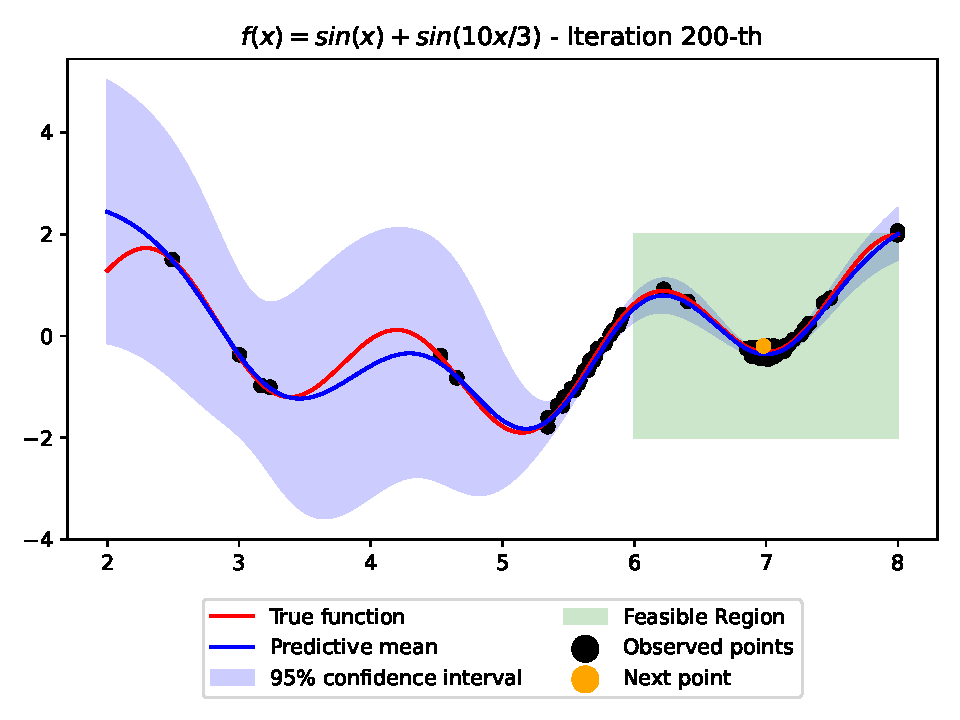
\includegraphics[width=\textwidth]{Figures/Neural-CBO/1d_toy.pdf}
    \caption{Minimization result with 1-D objective function $f(x) = \sin(x) + \sin(\frac{10x}{3})$ under the constraint $c(x) = (x-7)^2 -1 \le 0$}
    \label{fig:neural_cbo_toy_sample}
\end{figure}
In Figure \ref{fig:neural_cbo_toy_sample}, minimization result with 1-D objective function $f(x) = \sin(x) + \sin(\frac{10x}{3})$ under the constraint $c(x) = (x-7)^2 -1 \le 0$ is given to illustrate how variance formula in Eqn. \ref{Eqn:neural_cbo_variance_formula} and Alg. \ref{alg:neural_cbo} work. As shown in this figure, the variance formula performs well with relatively small values in feasible regions and larger values in infeasible regions. These results also demonstrate that the constraint model effectively guides our algorithm toward the feasible region, ensuring subsequent selection points remain within feasible regions and gradually approach the true minimum. 



\section{Theoretical Analysis}
To evaluate the performance of black-box optimization methods, much of the prior research on unconstrained \ac{bo} has focused on minimizing cumulative regret. As introduced in Section \ref{background:performance_metrics}, the cumulative regret after $T$ iterations is defined as:
\[
R_T = \sum_{t=1}^T r_t,  
\] 
where $r_t = f(\mathbf{x}_t) - f(\mathbf{x^*})$  represents the instantaneous regret, quantifying the difference between the value of the unknown function $f$ at the optimal point, $\mathbf{x}^* = \arg\max_{\mathbf{x} \in \mathcal{D}} f(\mathbf{x})$, and the value of the function at point $\mathbf{x}_t$, which is selected by the algorithm at iteration $t$. However, since $f(\mathbf{x^*})$ represents the optimal value under constraints, the algorithm may sometimes sample infeasible points with lower objective values than $f(\mathbf{x^*})$. To account for this, following \citet{xu2023constrained, nguyen2023optimistic}, we inherited the \textit{positive regret} definition as
$r_t^+ = [f(\mathbf{x}_t) - f(\mathbf{x^*})]^+,$
where $[\cdot]^+ \coloneqq \max\{0, \cdot\}$. Additionally, to measure constraint satisfaction, constraint \textit{violation} is defined as $
v_{c_i,t} = [c_i(\mathbf{x}_t)]^+$. 
Then, we introduce the \textit{cumulative positive regret} for the objective function, $R_T^+$, and the \textit{cumulative violation} for each constraint, $V_{c_i, T}$. These metrics measure the additional cost incurred due to suboptimal decisions and violations of the constraints over time by running the algorithm.  
\begin{definition} [Cumulative Positive Regret and Cumulative Violation]
    \begin{align*}
        R_T^+ &=\sum_{t=1}^T [f(\mathbf{x}_t) - f(\mathbf{x^*})]^+,
        \\
        V_{c_i, T}  &= \sum_{t=1}^T [c_i(\mathbf{x}_t)]^+, \forall i \in [K]
    \end{align*}
        
\end{definition}
\subsection{Detailed Assumptions for Objective Function and Constraints}

% \subsubsection{Assumption on black-box objective function and constraints}
We apply the general assumption stated in the Assumption \ref{assumption:rkhs} and \ref{assumption:subgaussian_noise} on both objective function and constraints:

\begin{itemize}
    \item \textbf{Objective function}: $f \in \mathcal{H}_{k_f}(\mathcal{D})$, $\norm{f}_{\mathcal{H}_{k_f}} \leq B$,  where $k_f$ is corresponding to $v(\cdot, \boldsymbol{\theta})$. The noisy observation at step $t$ is $y_t = f(\mathbf{x}_t) +  \epsilon_t$, where $\{\epsilon_i\}_{i=1}^t$ is sub-Gaussian with parameter $R_f$ and variance $\lambda_f$.

    \item \textbf{Constraint}: $c_i \in \mathcal{H}_{k_{c_i}}(\mathcal{D}), \norm{c_i}_{\mathcal{H}_{k_{c_i}}} \leq S_i$, where $k_{c_i}$ is corresponding to $u_{c_i}(\cdot, \boldsymbol{\omega}_{c_i}), \forall i = 1, \dots, K$. The noisy observation at step $t$ is $z_{c_i,t} = c_i(\mathbf{x}_t) + \eta_{c_i, t}$, where $\{\eta_{c_i, t}\}_{i=1}^t$ is sub-Gaussian with parameter $R_{c_i}$ and variance $\lambda_{c_i}$.
\end{itemize}
Now we can now state our main theorem:
\begin{restatable}{theorem}{TheoremMain}
\label{theorem:main}
    Under Assumption \ref{assumption:rkhs}, Assumption \ref{assumption:subgaussian_noise} and Condition \ref{condition:network_width}, set the step size used to train the neural networks in Alg. \ref{alg:neural_cbo} as $\alpha_t \le \frac{\nu}{(T+1)^2}$, then for any $\delta \in (0,1)$,  with probability at least $1 - \delta \exp (\Omega(C^{-L} m^{1/36}))$, the Cumulative Regret $R_T$ and Cumulative Violation $V_{c_i, T}$ after $T$ iterations are bounded as:
    \begin{align*}
        & V_{c_i, T} \le 2 \beta_{c_i,T} \sqrt{\frac{S_i T}{\log(S_i+1)} (2\gamma_{c_i,T}+1)} + 2\mathcal{E}(m),
        \\
        & R_T \le R_T^+ \le 2 \beta_{f,T} \sqrt{\frac{B T}{\log(B+1)} (2\gamma_{f,T}+1)} + 2 \mathcal{E}(m),
    \end{align*}
where $\mathcal{E}(m) = \mathcal{O}(C^{2L} L^{3/2} m^{11/36})$. Especially, by choosing $m = \Omega(d^9 \exp (\nu LC^L\log T)))$, the Cumulative Regret and Cumulative Violation enjoy the  following results:
\begin{align*}
        V_{c_i, T} = \mathcal{O}(\gamma_{c_i,T} \sqrt{T}), \;\;\;\;\; R_T = \mathcal{O}(\gamma_{f,T} \sqrt{T}).
    \end{align*}
\end{restatable}
\begin{remark}
Unlike previous works \citep{zhou2020neural, zhang2021neural} that require a neural network width of \( m = \Omega(T^6) \) for convergence when modeling the objective function, our analysis builds on recent analyses from \citet{xu2024overparametrized}, which show that only a linear condition of \( m = \Omega(T) \) is needed. Furthermore, while \citet{xu2024overparametrized} focus on the input domain \( \mathbb{S}^{d-1} \), we can adapt to inputs \( \mathbf{x} \in \mathbb{R}^d \) with \( 0 < n_l < \|\mathbf{x}\| < n_b \) (where \( n_l \) and \( n_b \) are positive constants) without changing the order of \( T \) in the width condition for \( m \). Similar arguments are noted in \citep{du2018gradient, cao2020generalization}.
\end{remark}

\section{Experiments}
\label{section:neural-cbo_exp}
In this section, we outline and discuss our experimental results. We apply our method to synthetic, real-world functions. Our implementations of both problems are available at: \url{https://github.com/phantrdat/neural-cbo}.
\subsection{Experimental Setup}
\label{section:neural-cbo_baselines}
For all experiments, we compared our algorithm with well-known Constrained \ac{ei} (cEI), the extension of \ac{ei} into constrained \ac{bo} from \citet{gardner2014bayesian}. Besides, we also compare our algorithm with recent state-of-the-art algorithms in unknown constrained \ac{bo}, including ADMMBO \citep{ariafar2019admmbo}, UCB-C \citep{nguyen2023optimistic} and ConfigOpt \citep{xu2023constrained}. For our proposed Neural-CBO algorithm, we employ fully connected deep neural networks as the surrogate models for both objective function and constraints. Implementation details of our Neural-CBO algorithm as well as baselines are as follows:
\begin{itemize}
    \item  \textbf{Constrained EI} (cEI) \citep{gardner2014bayesian} integrates feasibility into the acquisition function by multiplying the probability of feasibility into EI value at every point in the search space.
    \item \textbf{ConfigOpt} \citep{xu2023constrained}: Optimize LCB-based acquisition function for the objective, which satisfies LCB-based conditions for constraints. For cEI and ConfigOpt, we used the public implementation provided at GitHub repository: \url{https://github.com/PREDICT-EPFL/ConfigOPT}.
    \item \textbf{ADMMBO} \citep{ariafar2019admmbo}: Reformulates the constrained optimization problem into an unconstrained one using the Alternating Direction Method of Multipliers (ADMM) framework. As the official implementation of ADMMBO is written in Matlab and available at \url{https://github.com/SetarehAr/ADMMBO}, we use our own Python implementation based on the official implementation.  
    \item \textbf{UCB-C} \citep{nguyen2023optimistic}: 
    Similar to ConfigOpt, but using a UCB-based acquisition function for the objective, we utilized the implementation obtained directly from the authors.
\end{itemize}
\paragraph{Neural-CBO implementation details:}
As described in Section \ref{section:neural-cbo}, the network's weights are initialized with independent samples drawn from a normal distribution $\mathcal{N} (0, 1)$. We also initialize fixed outer weight $\mathbf{q}$ to be a symmetric Bernoulli random variable with equal probability to be $-1$ or $1$. To train the surrogate neural network models, we use a Gradient Descent optimizer described in the main paper with a learning rate $\alpha = 0.001$. The network width depends on the tasks and is set to be $m = T$, where $T$ is the number of optimization iterations. We choose the network depth $L=2$ to reduce computational costs. 

\subsection{Synthetic Benchmark Functions}
\label{section:neural-cbo_synthetic}
We conducted optimization experiments on four synthetic objective functions: Branin, Ackley, Simionescu and Hartmann. The input dimension of each objective function and the corresponding number of constraints are summarized in Table \ref{table:synthetic_info}. Due to space limitations, we present the expression of each function and its constraints in the Supplementary material. 
  \begin{table}[h]
  \centering
 \caption{The input dimension and number of constraints for each synthetic objective function.}
 \vspace{0.15in}
\begin{tabular}{|c|c|c|c|c|c|}
\hline
\textbf{Obj}              & Branin & Simionescu & Ackley & Hartmann  \\ \hline
\textbf{Dim}                   & 2   & 2               & 5 & 6                  \\ \hline
\textbf{Constraints}       & 1      & 1              & 2       & 1          \\ \hline
\end{tabular}
\label{table:synthetic_info}
\end{table}
% \looseness=-1
The noise in function evaluations follows a normal distribution with zero mean, and the variance is set to 1\% of the function range. All experiments reported here are averaged over 20 runs, each with random initialization. We report the (Log10 of) the Best Positive Regret plus Violation in Figure \ref{fig:neural-cbo_synthetic}

To ensure statistical significance, we performed one-sided $t$-tests to assess whether a baseline outperforms Neural-CBO in terms of the best positive regret plus violation. The null hypothesis is $H_0: \mu_\text{baseline} \leq \mu_{\text{Neural-CBO}}$, and the alternative hypothesis is $H_a: \mu_\text{baseline} > \mu_{\text{Neural-CBO}}$, where $\mu_\text{baseline}$ and $\mu_{\text{Neural-CBO}}$ represent the means of the (Log10 of) Best Positive Regret plus Violation values of the baseline and our proposed Neural-CBO, respectively. Note that lower values indicate better performance. We present the statistical test results for four synthetic benchmark functions and two real-world tasks (described in Section \ref{section:neural-cbo_gas} and \ref{section:neural-cbo_speed}) in Table \ref{table:t-test}. Each cell in the table shows the $p$-value from the $t$-test as the first value. To account for multiple comparisons, the Benjamini-Hochberg correction was applied, with the corrected value provided as the second value. A result is labeled as ``T'' if the null hypothesis is rejected, meaning that Neural-CBO is statistically better to the compared baselines. Conversely, a result is labeled ``F'' if we cannot reject the null hypothesis, meaning that the baselines and the Neural-CBO are comparable.
\begin{table}[ht]
\caption{One-sided $t$-tests to evaluate whether the baseline outperforms Neural-CBO in terms of the best positive regret plus violation.}
  \vspace{0.15in}
\resizebox{\linewidth}{!}{
\begin{tabular}{|l|c|c|c|c|}
\hline
\multicolumn{1}{|c|}{\textbf{}} & \textbf{ConfigOpt} & \textbf{cEI}  & \textbf{UCB-C} & \textbf{ADMMBO} \\ \hline
\textbf{Branin}             & (8.25e-06, T)      & (6.41e-20, T) & (4.68e-73, T)     & (6.86e-102, T)  \\ \hline
\textbf{Simionescu}             & (6.19e-07, T)      & (2.42e-13, T) & (2.13e-25, T)  & (1.32e-78, T)   \\ \hline
\textbf{Ackley}                 & (6.95e-29, T)      & (0.13, F)      & (6.4e-97, T)   & (0.21, F)        \\ \hline
\textbf{Hartmann}               & (0.00594, T)       & (1.54e-59, T) & (4.88e-118, T) & (1.2e-87, T)    \\ 
\hline
\textbf{Gas Transmission}               & (1.52e-46, T)       & (1.78e-48, T) & (1.66e-25, T) & (1.54e-73, T)    \\ 
\hline
\textbf{Speed Reducer}               & (0.77, F)       & (6.99e-74, T) & (5.22e-77, T) & (0.38, F)    \\ 
\hline
\end{tabular}
\label{table:t-test}
}
\end{table}


\begin{figure}[h]
    \centering
   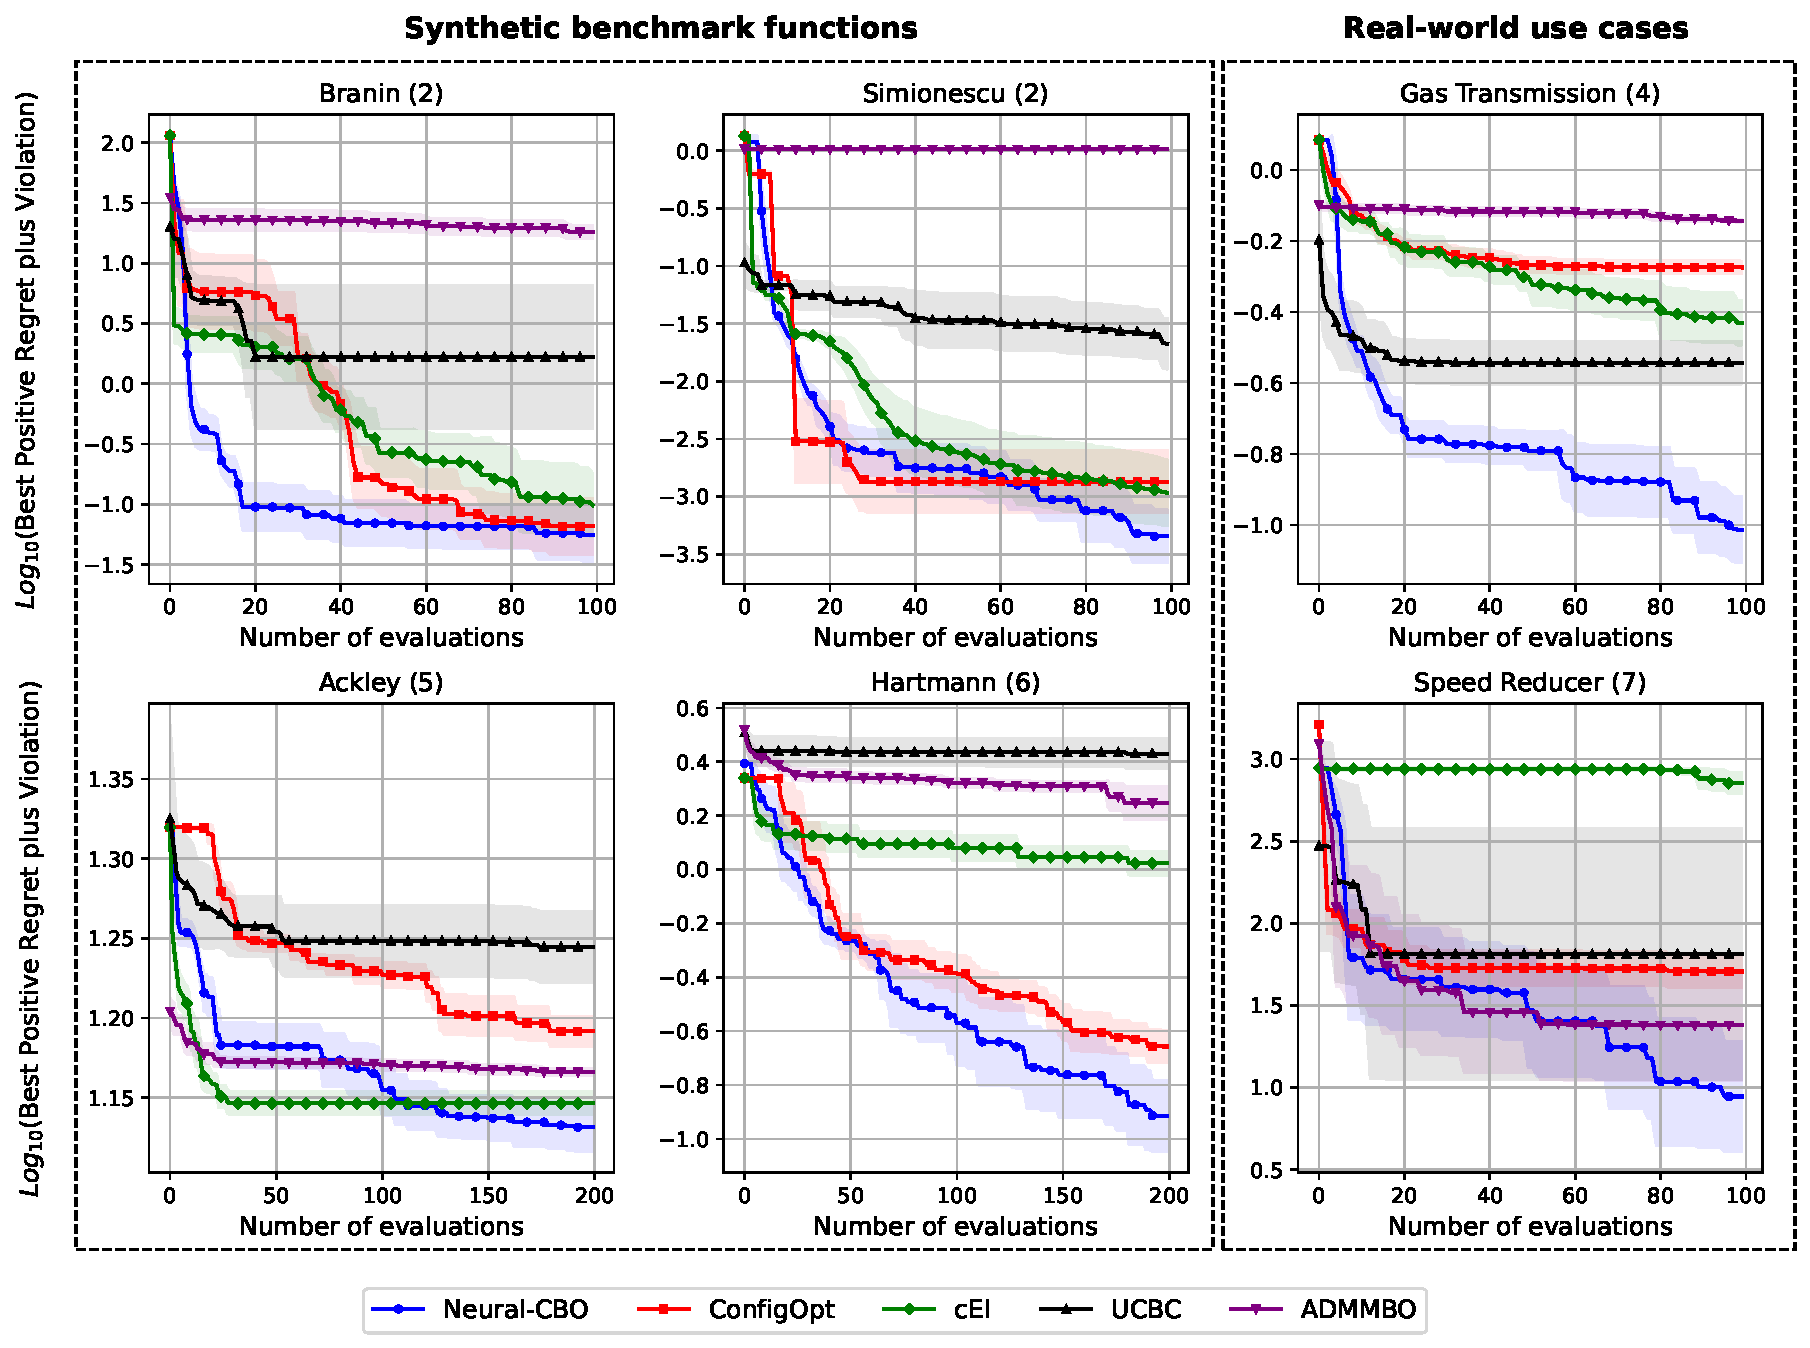
\includegraphics[width=\textwidth]{Figures/Neural-CBO/Branin-Simionescu-GasTransmission-Ackley-Hartmann-SpeedReducer.pdf}
   % \vspace{0.15in}
    \caption{The plots show (Log10 of) the Best Positive Regret plus Violation up to step $t$, which is $\min_{t \in [T]} [f(\mathbf{x}_t) - f^*]^+ + \sum_{k=1}^K [c_k(\mathbf{x}_t)]^+ ]$, comparing our proposed algorithm and four baselines. The dimension of each objective function is shown in the parenthesis. The left group is four synthetic functions introduced in Section \ref{section:neural-cbo_synthetic}, while the right group is the optimization results of Gas Transmission Compressor Design and Speed Reducer Design, described in Section  \ref{section:neural-cbo_gas} and \ref{section:neural-cbo_speed}.}
    
    \label{fig:neural-cbo_synthetic}
\end{figure}

We analyse three real-world constrained black-box optimization tasks: gas transmission compressor and speed reducer designs from \citet{kumar2020test}, and a third inspired by \citet{he2018verideep}. Details of each task will follow in the upcoming sections.  
\subsection{Gas Transmission Compressor Design}
\label{section:neural-cbo_gas}
     The main objective is to minimize operational costs or energy consumption. This requires identifying the optimal configuration of the compressor by optimizing four design variables. The problem involves $d = 4$ input dimensions and includes $K = 1$ constraint. The mathematics formula for this problem is:
    \begin{align*}
        f(\mathbf{x}) & = 8.61 \times 10^5\mathbf{x}_1^{1/2} \mathbf{x}_2\mathbf{x}_3^{-2/3} \mathbf{x}_4^{-1/2}  + 3.69 \times 10^4\mathbf{x}_3 + 7.72 \times 10^8 \mathbf{x}_1^{-1} \mathbf{x}_2^{0.219} \\
        & \;\;\; \; - 765.43 \times 10^6\mathbf{x}_1^{-1},
        \\
        \text{s.t }  c(\mathbf{x}) &= \mathbf{x}_4\mathbf{x}_2^{-2} + \mathbf{x}_2^{-2} - 1 \le 0
    \end{align*}

    
 \subsection{Speed Reducer Design}
\label{section:neural-cbo_speed}
This task involves designing a speed reducer for a small aircraft engine, focusing on minimizing weight while meeting several constraints, including bending stress on gear teeth, surface stress, transverse deflections of shafts, and shaft stresses. The problem includes 7 decision variables and 11 constraints, resulting in an input dimension of $d=7$ and $K=11$ constraints and can be formulated as:
\begin{align*}
    f(\mathbf{x}) &= 0.7854\mathbf{x}_2
^2 \mathbf{x}_1(14.9334\mathbf{x}_3 - 43.0934 + 3.3333\mathbf{x}_3^2) 
\\
    & \;\;\;\; +0.7854(\mathbf{x}_5\mathbf{x}_7^2 + \mathbf{x}_4\mathbf{x}_6^2) - 1.508\mathbf{x}_1(\mathbf{x}_7^2 + \mathbf{x}_6^2) + 7.477(\mathbf{x}_7^3 + \mathbf{x}_6^3), 
    \\
    \text{s.t. } & \begin{cases} 
    c_1(\mathbf{x}) = -\mathbf{x}_1\mathbf{x}_2^2\mathbf{x}_3 + 27  & \le 0 
    \\
    c_2(\mathbf{x}) = -\mathbf{x}_1\mathbf{x}_2^2\mathbf{x}_3^2 + 397.5 & \le 0 
    \\
    c_3(\mathbf{x}) = -\mathbf{x}_2\mathbf{x}_6^4
    \mathbf{x}_3\mathbf{x}_4^{-3}+ 1.93 &\le 0 
    \\
    c_4(\mathbf{x}) = -\mathbf{x}_2\mathbf{x}_7^4
    \mathbf{x}_3\mathbf{x}_5^{-3}+ 1.93 & \le 0 
    \\
    c_5(\mathbf{x}) = 10\mathbf{x}_6^{-3} \sqrt{16.91 \times 10^6 + (745\mathbf{x}_4\mathbf{x}_2^{-1}
    \mathbf{x}_3^{-1}
    )^2} -1100 & \le 0
    \\
    c_6(\mathbf{x}) = 10\mathbf{x}_7^{-3} \sqrt{157.5 \times 10^6 + (745\mathbf{x}_5\mathbf{x}_2^{-1}
    \mathbf{x}_3^{-1}
    )^2} - 850 & \le 0
    \\
    c_7(\mathbf{x}) = \mathbf{x}_2\mathbf{x}_3 -40 & \le 0 
    \\
    c_8(\mathbf{x}) = -\mathbf{x}_1 \mathbf{x}_2^{-1} + 5 & \le 0
    \\
    c_9(\mathbf{x}) = -\mathbf{x}_1 \mathbf{x}_2^{-1} - 12  & \le 0
    \\
    c_{10}(\mathbf{x}) = 1.5\mathbf{x}_6 - \mathbf{x}_4  + 1.9  & \le 0
    \\
    c_{11}(\mathbf{x}) = 1.1\mathbf{x}_7 - \mathbf{x}_5  + 1.9  & \le 0
    \\
    \end{cases},
\end{align*}

We report numerical results of Section \ref{section:neural-cbo_gas} and  \ref{section:neural-cbo_speed} in Figure \ref{fig:neural-cbo_synthetic} and Table \ref{table:t-test}.
\subsection{Designing Sensitive Samples for Detection of Model Tampering}
\label{section:neural-cbo_sensitive_sample}
\begin{figure}[H]
    \centering
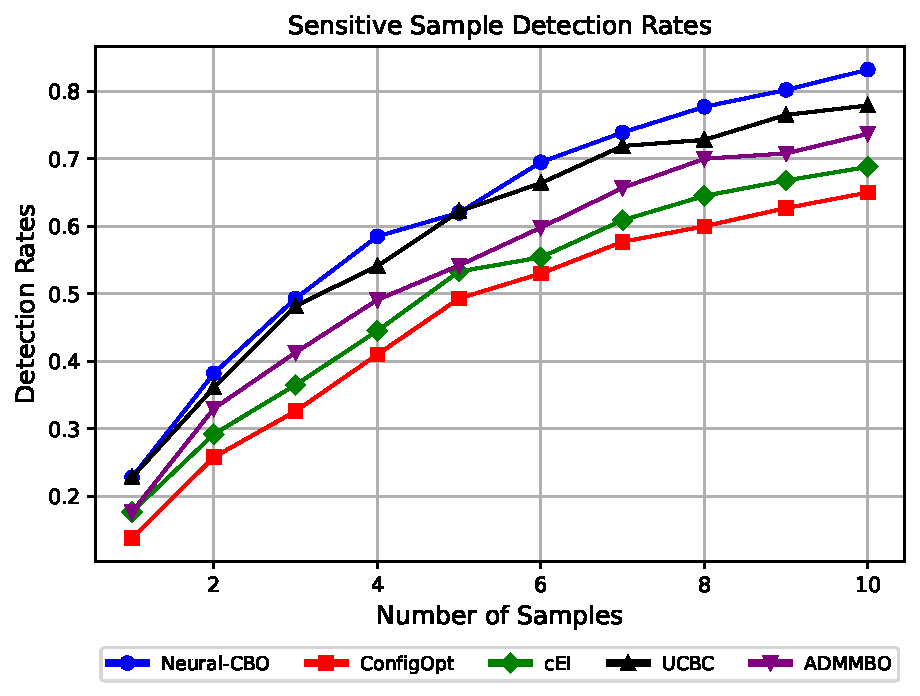
\includegraphics[width=\textwidth]{Figures/Neural-CBO/sensitive_sample_detection_rate.pdf}
    \caption{ \textbf{Detection Rates} corresponding to the number of samples on the MNIST dataset. As shown in the figure, Neural-CBO can generate sensitive samples that achieve nearly 85\% of the detection rate with at least 10 samples.}
    \label{fig:sensitive_sample}
\end{figure}

We build on the sensitive sample generation example described in Section \ref{section:neural-bo_sensitive_samples} to address an additional practical challenge: incorporating constraints on the generated samples to ensure their realism. Specifically, in scenarios where tampered machine learning models are hosted on cloud services, attackers may attempt to bypass detection by modifying models while keeping their behavior on plausible inputs unchanged. To prevent attackers from evading detection, sensitive samples must resemble normal inputs. Therefore, a human-in-the-loop process is employed, where reviewers rate the realism of each sample on a scale of $(0,1)$; higher scores indicate more realistic samples. These scores serve as constraints in the optimization, where obtaining human feedback can be costly. Assuming a pre-trained model $s_\varphi(\mathbf{x})$ may have been altered after being uploaded, the goal is to find sensitive samples by solving the optimization problem: 
\begin{align*}
    v &= \argmax_\mathbf{x} \norm{\frac{\partial s_\varphi(\mathbf{x})}{\partial \varphi}}_F 
    \\
    \text{s.t. } &  realistic(v) \ge h, 
\end{align*}
where $\norm{\cdot}_F$ denotes the Frobenius norm, $realistic(\cdot)$ is the human-based scoring function and $h$ is a pre-defined threshold. A detection is \emph{successful} if at least one of the $N_S$ sensitive samples shows a different top-1 prediction between the tampered and original models.  

We employed the same experimental setup outlined in Section \ref{section:neural-bo_sensitive_samples}, using a pre-trained MNIST handwritten digit classification model and compared our method's performance against several baselines based on average detection rates for sensitive samples. The model was tampered with by adding noise to its weights 1,000 times, producing 1,000 distinct versions. While the original model had a top-1 accuracy of 93\%, this dropped to $87.73\% \pm 0.08\%$ after tampering. To reduce computational costs, we downscaled the images from $28 \times 28$ to $7 \times 7$, optimized in this 49-dimensional space, and then restored them to the original resolution to generate sensitive samples. Feasible samples were chosen based on their realistic scores. Figure \ref{fig:sensitive_sample} shows the detection rates of (feasible) sensitive samples generated by our method compared to four baselines, demonstrating that our samples achieved higher detection rates. As expected, the detection rate improves with more samples and our method is consistently competitive.







\section{Conclusion}
We proposed a novel algorithm for black-box optimization with unknown constraints, utilizing deep neural networks as surrogate models for both the objective function and constraints. Our algorithm leverages the bounded nature of constraint values by applying LCB conditions at each iteration to ensure feasibility. We also employ EI as the acquisition function to balance exploration and exploitation, especially in scenarios where feasible regions are significantly smaller than the search space. Our theoretical analysis shows that, under mild conditions regarding neural network width, our algorithm achieves upper bounds on cumulative regret and constraint violations comparable to previous GPs-based methods. We validate our approach through experiments on synthetic and real-world benchmark tasks involving structural data, with results demonstrating competitive performance against state-of-the-art methods.

% as our baseline and tampered it by adding noise to each weight 1,000 times, resulting in 1,000 distinct models. The original model had a top-1 accuracy of $93\%$, which dropped to $87.73\% \pm 0.08\%$ after tampering. To reduce computational costs, we downscaled the images from $28 \times 28$ to $7 \times 7$, optimizing in this 49-dimensional space. After identifying the optimal points, we restored them to the original resolution to generate sensitive samples.
